\documentclass[11pt,a4paper]{article}
\usepackage[margin=2.4cm]{geometry}
\usepackage{times}
\usepackage{graphicx}
\usepackage{booktabs}
\usepackage{xcolor}
\usepackage{hyperref}
\usepackage{titlesec}
\usepackage{setspace}
\usepackage{caption}

\definecolor{ink}{HTML}{1a1a1a}
\definecolor{rulec}{HTML}{2060cc}
\hypersetup{colorlinks=true,linkcolor=rulec,citecolor=rulec,urlcolor=rulec}

\titleformat{\section}{\large\bfseries\color{ink}}{\thesection}{0.7em}{}[\vspace{-0.4em}{\color{rulec}\titlerule[0.6pt]}]
\titleformat{\subsection}{\normalsize\bfseries\color{ink}}{\thesubsection}{0.6em}{}
\titlespacing*{\section}{0pt}{1.3em}{0.55em}

\captionsetup{font=small,labelfont=bf,skip=6pt}
\setstretch{1.15}
\pagestyle{plain}

\begin{document}
\begin{center}
{\scriptsize\color{rulec}\textbf{DRAFT v0.3 \quad ACM Digital Government: Research and Practice \quad practice paper}}\\[0.7em]
{\LARGE\bfseries Grouping Duplicate Citizen Complaints\\[0.15em] in a State Ombudsman}\\[0.45em]
{\large\textit{A first operational account from Cear\'{a}, Brazil}}\\[0.9em]
Berg Silva, Charles, Ana Luiza Cruz, and Francisco Nauber Bernardo Gois\textsuperscript{*}\\[0.25em]
{\small Controladoria e Ouvidoria Geral do Estado do Cear\'{a} (CGE-CE), Fortaleza, Brazil}\\[0.15em]
{\small\textsuperscript{*}francisco.gois@cge.ce.gov.br}\\[0.7em]
{\small 23 September 2026 \textperiodcentered\ not submitted \textperiodcentered\ authorship provisional}
\end{center}

\vspace{0.4em}
\noindent\textbf{Abstract.}
State ombudsman offices receive many complaints that tell the same story in different words. Officers then open several files for one event. Similaridade is the system used by CGE-CE to group those texts before a human links them. This practice paper reports the method in production in August 2026 and a homolog test of a later stack on the same 4{,}389 real complaints.

The production pipeline encodes each complaint with TF-IDF and groups neighbors with DBSCAN. A cluster is kept only when mean intra-cluster cosine similarity is at least 0.75. On that batch the production stack grouped 62.4\% of texts. A homolog stack that uses sentence embeddings, HDBSCAN, and a reasoning model on leftovers grouped 84.9\% (3{,}725 complaints in 354 clusters). An LLM pass recovered 104 of 768 leftovers into 21 themes. About 87\% of the grouped items fell in a green band meant for bulk linking, which would leave officers with roughly 484 cases to inspect instead of 3{,}725.

The new stack is not a finished production claim. Short complaints still yield weak vectors. In September 2026 the live job at times collapsed to a single cluster. The Ouvidoria has not yet labeled a held-out sample.

\noindent\textbf{Keywords:} citizen complaints; ombudsman; text clustering; sentence embeddings; HDBSCAN; digital government; Brazil

\vspace{0.3em}
{\color{rulec}\hrule height 0.6pt}
\vspace{1em}

\section{Introduction}
An ombudsman file starts as free text. The same broken pipe, the same delay at a public counter, or the same coordinated campaign can arrive tens of times in one morning. If each arrival becomes its own case, the officer repeats the same reading and the citizen waits longer.

Similaridade is CGE-CE's answer to that pile. It runs on the complaint stream of the state Ouvidoria (COUVI). The job is narrow: put texts that likely refer to the same event in one group, mark the rest as leftovers, and show the officer a band (green, yellow, red) instead of a raw list.

Most recent public-sector NLP work classifies a complaint into a department or extracts a theme. Similaridade does something closer to duplicate detection: it asks whether two texts are the same case. The contribution of a later version, if it holds, is an operational account: one Brazilian state stream, two stacks on the same 4{,}389 complaints, and a triage rule that cuts the reading load.

\section{State of the art}
Public grievance research splits into three jobs that are easy to mix up.

\textbf{Routing and classification.}
Das et al.\ built a decision-support redressal system that used sentence-level sentiment to help officers triage incoming text~\cite{das2020grievance}. Rakhimzhanov, Belginova, and Yedilkhan compared large language models with instruction-tuned embeddings on municipal transport complaints. Fine-tuned embeddings reached about 90\% accuracy and were cheaper to run than prompting an LLM for every item~\cite{rakhimzhanov2025transport}. That result matters for Similaridade: the expensive model should see leftovers, not the whole stream.

\textbf{Theme discovery.}
BERTopic embeds documents, reduces them, clusters with HDBSCAN, and labels each cluster with class-based TF-IDF~\cite{grootendorst2022bertopic}. Tang, Pan, and Gu used that recipe on China's online government inquiry platform~\cite{tang2024bertopic}. Theme models are useful for policy. They are the wrong metric when an officer must link copy-paste waves that share one event and many wordings.

\textbf{Semantic grouping of complaints.}
Esperan\c{c}a et al.\ applied BERT sentence embeddings and clustering to informatics complaints in a Portuguese public agency, then put the groups on a live dashboard~\cite{esperanca2025complaint}. Their target is still a category. Ours is a case: two texts about the same water outage should share a group even if the theme ``water'' already exists.

Table~\ref{tab:sota} places the stacks against that map. Production Cear\'{a} is lexical near-duplicate detection. The homolog stack is the BERTopic family (embeddings + HDBSCAN) plus an LLM only on leftovers. The missing piece is a human label of ``same case'' from ombudsman officers.

\begin{table}[ht]
\centering
\caption{Recent public-sector complaint work versus Similaridade.}
\label{tab:sota}
\small
\begin{tabular}{llll}
\toprule
Work & Task & Representation & Grouping \\
\midrule
Das et al.\ (2020) & Route / triage & Sentiment features & Supervised \\
Tang et al.\ (2024) & Theme & Embeddings & BERTopic \\
Rakhimzhanov et al.\ (2025) & Route & E5 / BGE / LLM & Classifier \\
Esperan\c{c}a et al.\ (2025) & Theme / pattern & BERT embeddings & Semantic clusters \\
Similaridade (production) & Case & TF-IDF & DBSCAN \\
Similaridade (homolog) & Case & Sentence embeddings & HDBSCAN + LLM \\
\bottomrule
\end{tabular}
\end{table}

On the method side the genealogy is short. Term weights still catch identical paste~\cite{salton1988term}. DBSCAN finds dense regions and treats sparse points as noise~\cite{ester1996dbscan}. HDBSCAN drops the fixed radius~\cite{campello2013hdbscan}. Sentence-BERT gives vectors that cosine can compare without a cross-encoder on every pair~\cite{reimers2019sbert}.

\section{Setting}
CGE-CE is the state controller and ombudsman of Cear\'{a}. Similaridade serves the Ouvidoria. ASESI builds and runs the software. Airflow starts the job three times a day (08:00, 12:00, 17:00). Complaint text is sensitive. We report only aggregate counts. No complaint body is reproduced.

\section{Methods}
Figure~\ref{fig:pipeline} shows the two stacks on the same incoming text.

\begin{figure}[ht]
\centering
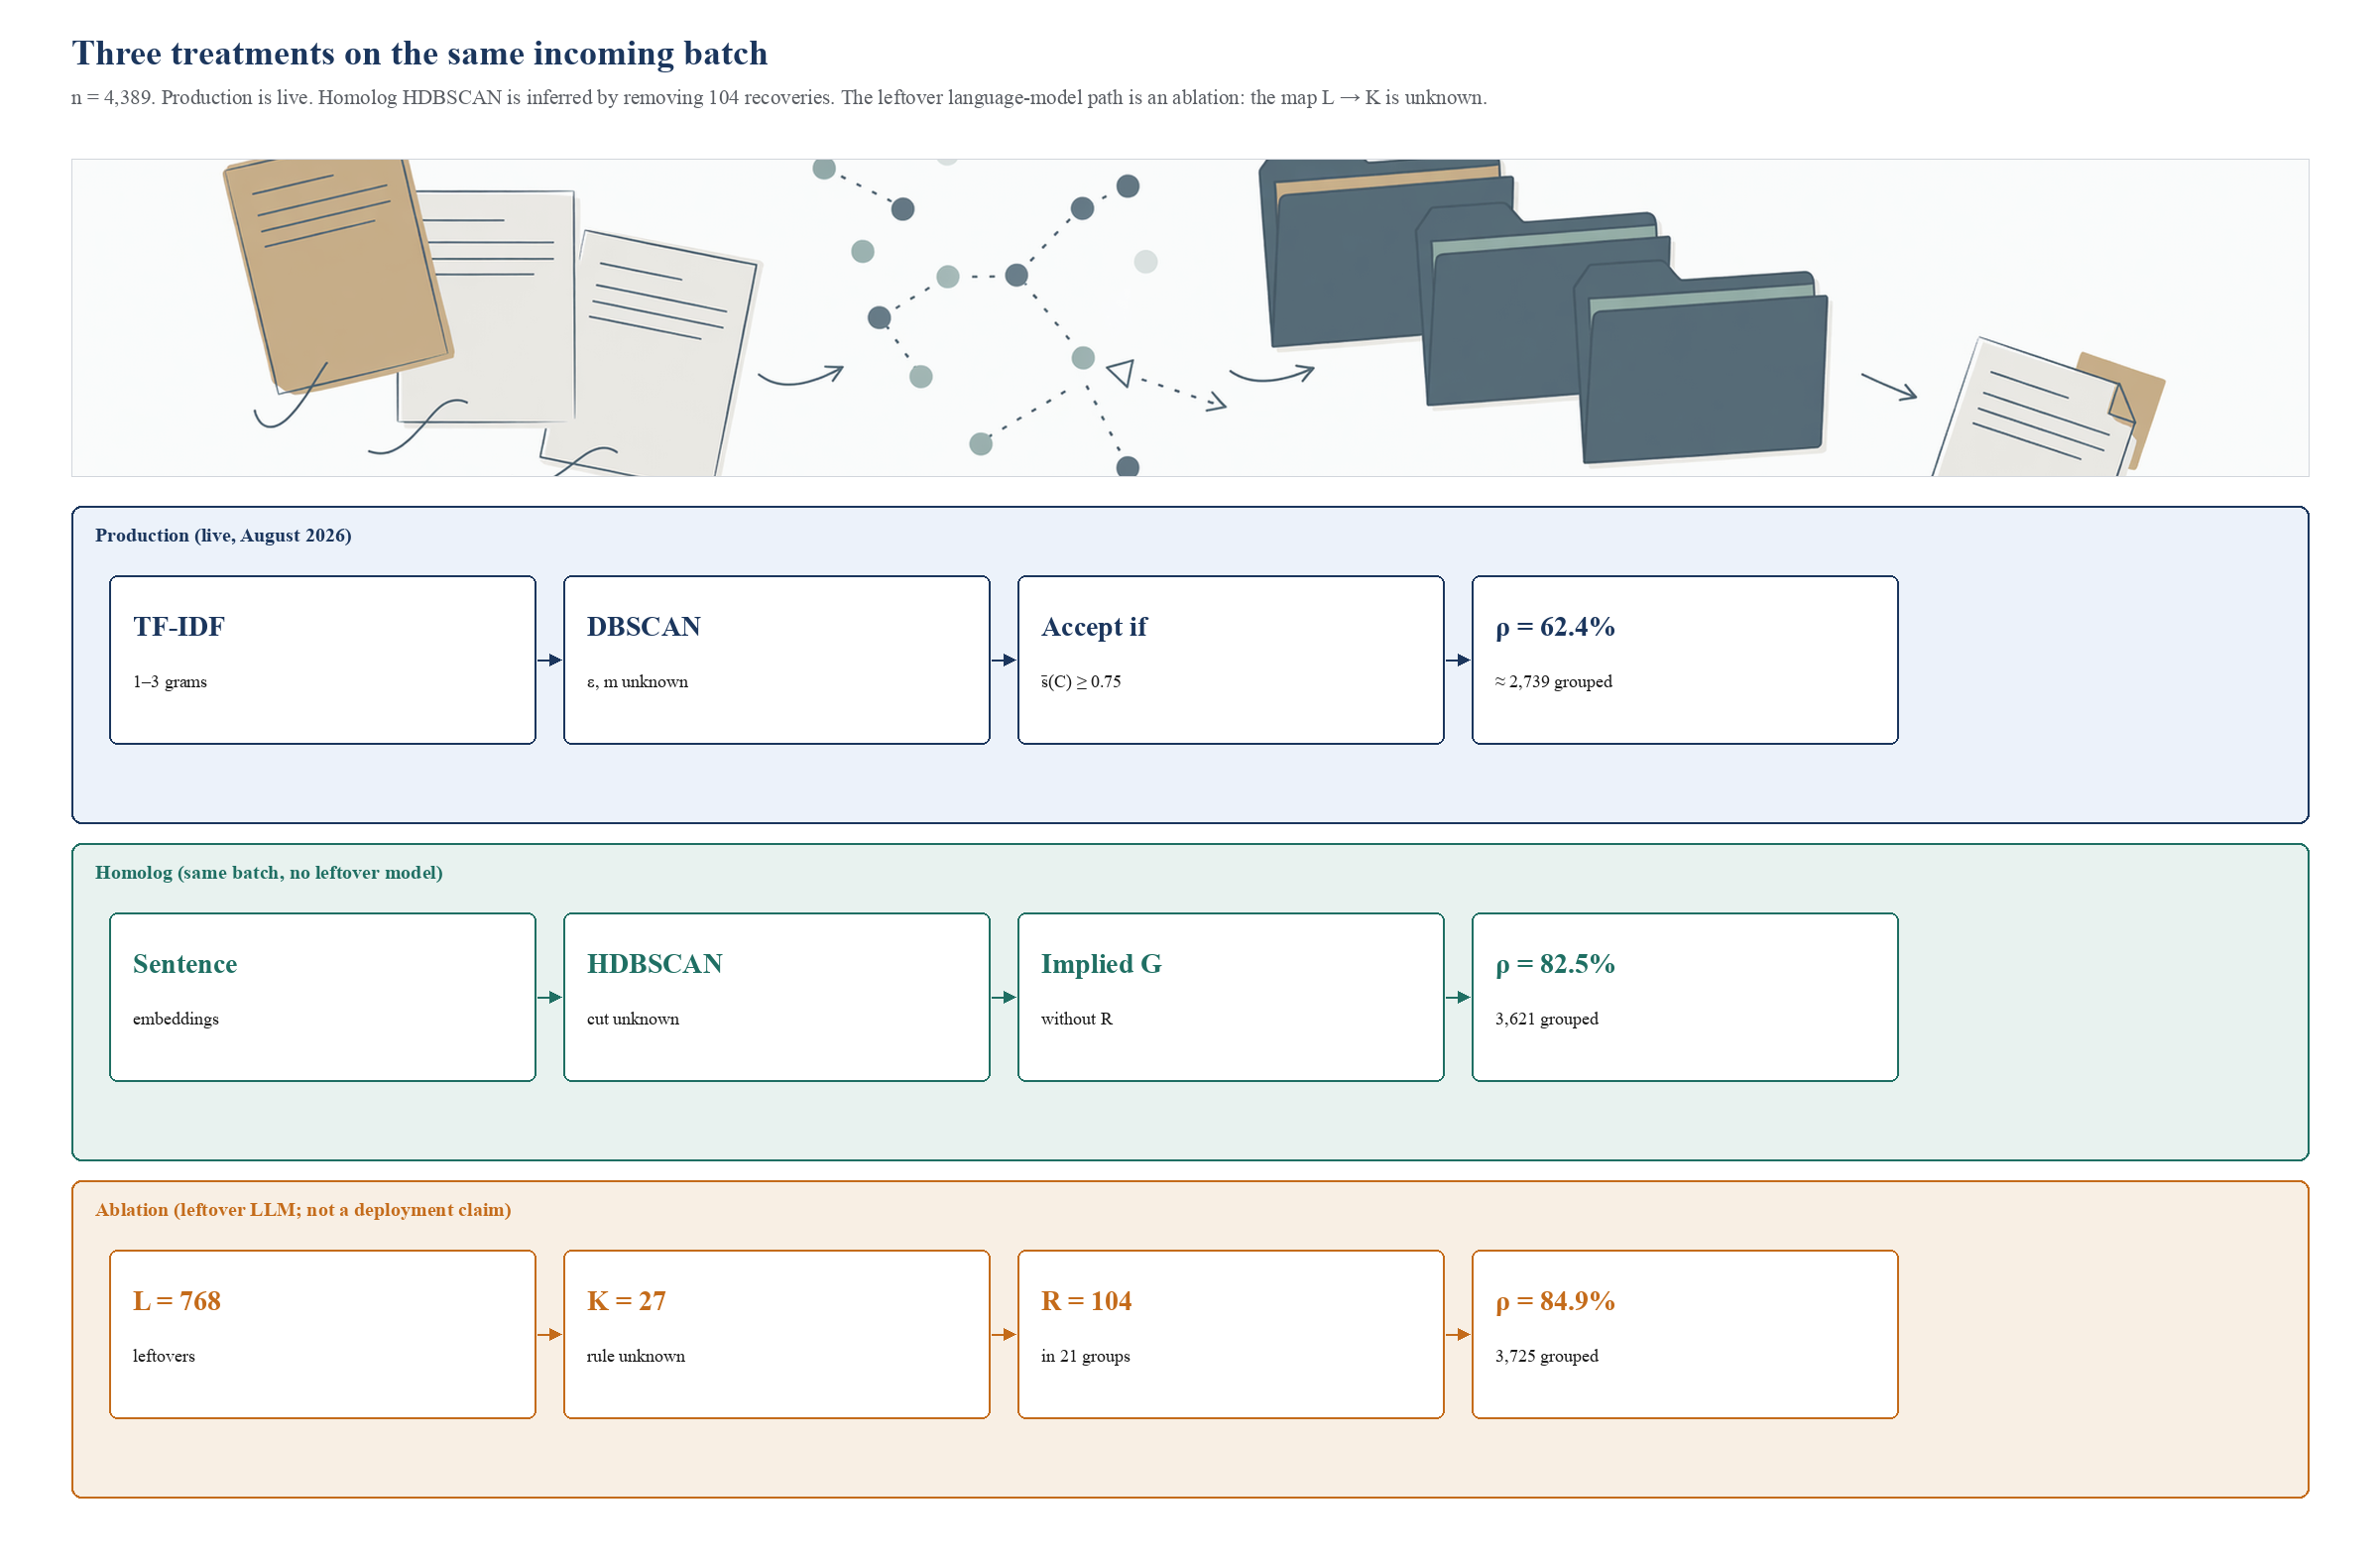
\includegraphics[width=\textwidth]{figures/fig1_pipeline.png}
\caption{Two pipelines on the same complaint stream. Production (top) is lexical. Homolog (bottom) embeds the text, clusters without a fixed radius, and spends the LLM only on leftovers.}
\label{fig:pipeline}
\end{figure}

\textbf{Production.} TF-IDF over unigrams, bigrams, and trigrams; $L_2$-normalized vectors; DBSCAN; keep a group only if mean pairwise cosine similarity $\ge 0.75$. Similarity is not transitive: $A$ can sit close to $B$ and $B$ to $C$ while $A$ and $C$ score near 0.006 and still share a label.

\textbf{Homolog.} Sentence embeddings, HDBSCAN, then DeepSeek R1 on a reduced leftover list. About 4{,}000 complaints encoded in a little over three minutes.

\textbf{Operator bands.} Green (bulk linking), yellow (confirm), red (read with care). 100\% internal similarity means identical texts.

\section{Results}
Both rows in Figure~\ref{fig:rate} use the same 4{,}389 real complaints. Production grouped 62.4\%. Homolog grouped 84.9\% (3{,}725 complaints in 354 clusters).

\begin{figure}[ht]
\centering
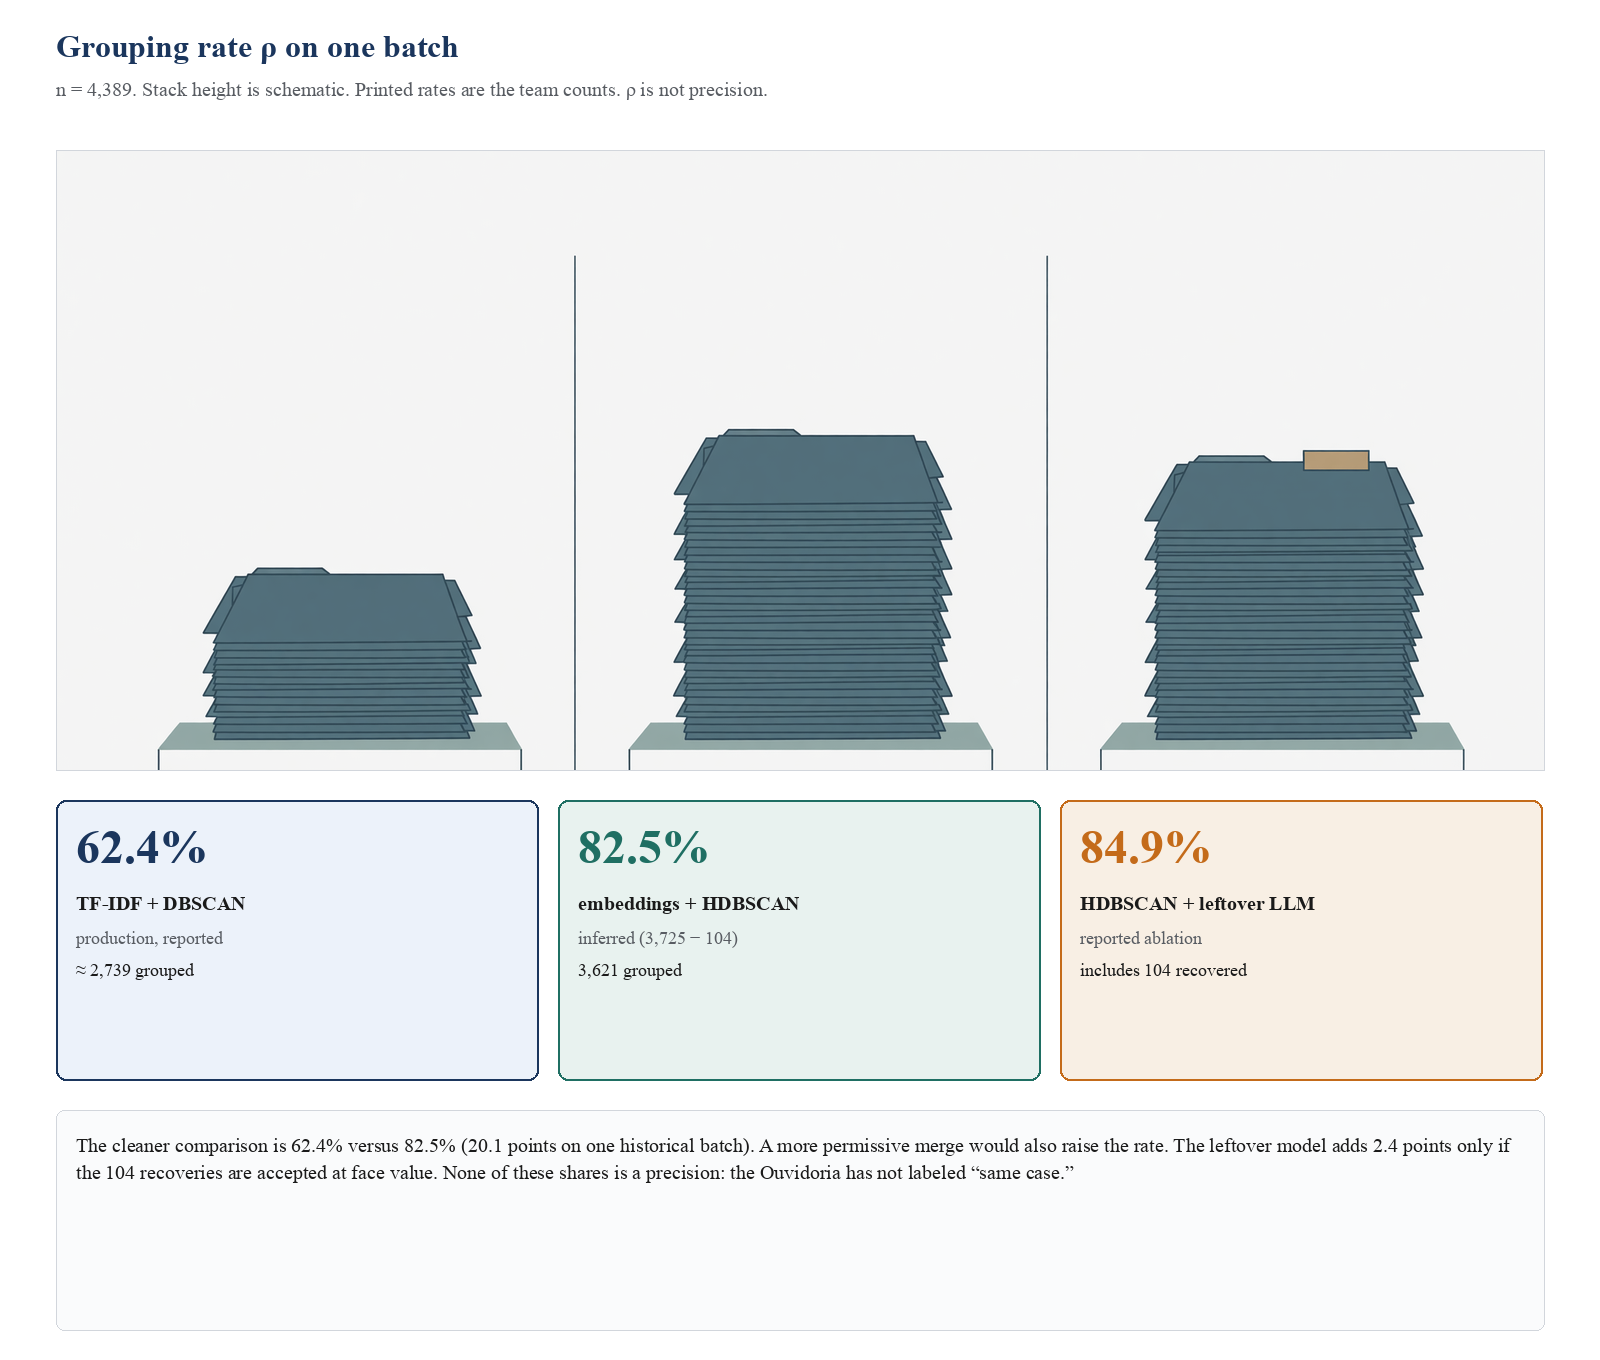
\includegraphics[width=0.72\textwidth]{figures/fig2_grouping_rate.png}
\caption{Share of the 4{,}389-complaint batch placed in a group.}
\label{fig:rate}
\end{figure}

The leftover path is in Figure~\ref{fig:funnel}: 768 ungrouped, 27 candidates, 104 recovered, 21 themes. About 87\% of grouped items sat in the green band, leaving roughly 484 cases for the officer (Figure~\ref{fig:load}).

\begin{figure}[ht]
\centering
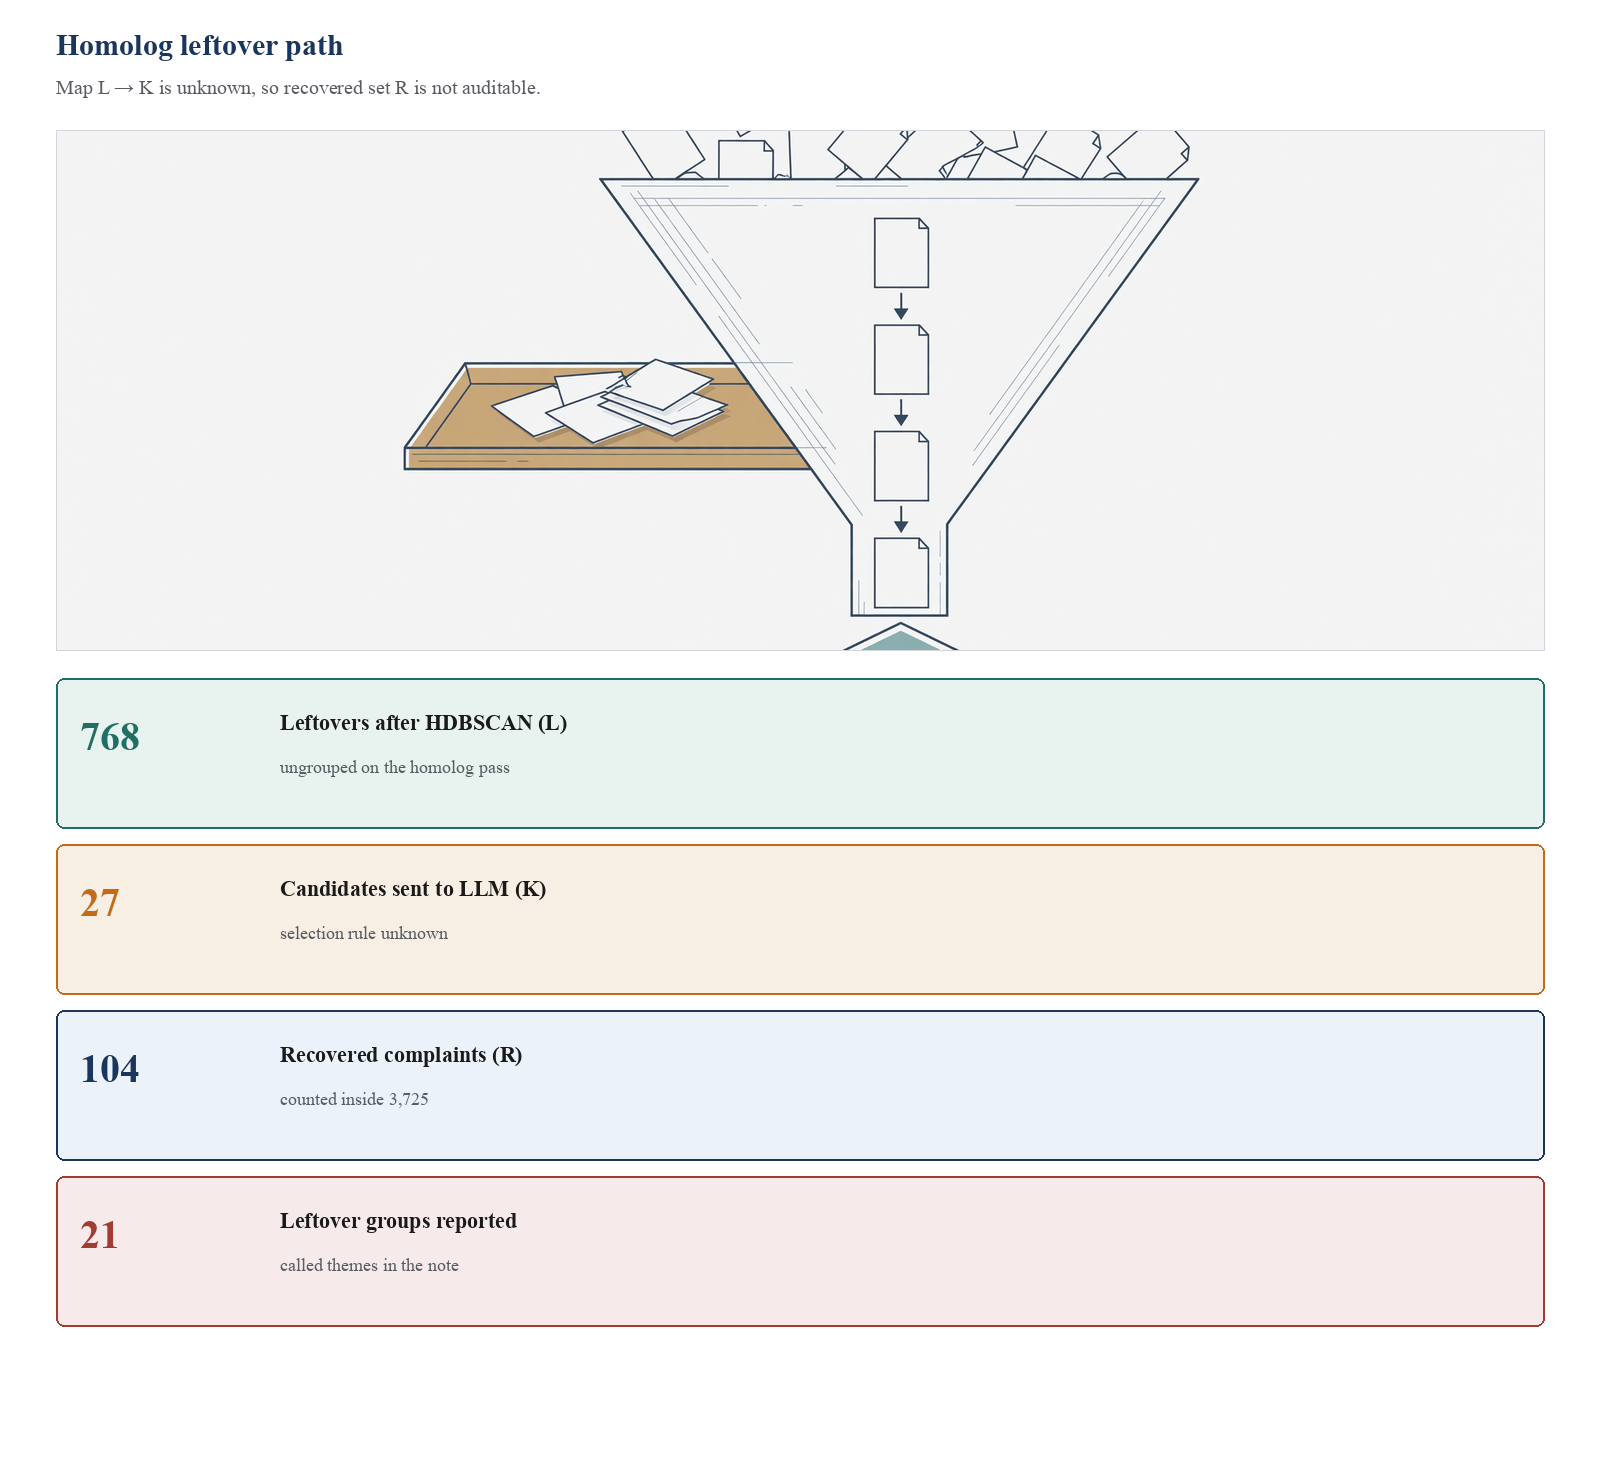
\includegraphics[width=0.78\textwidth]{figures/fig3_outlier_funnel.png}
\caption{Homolog leftover path. How the 27 candidates were chosen is not yet documented.}
\label{fig:funnel}
\end{figure}

\begin{figure}[ht]
\centering
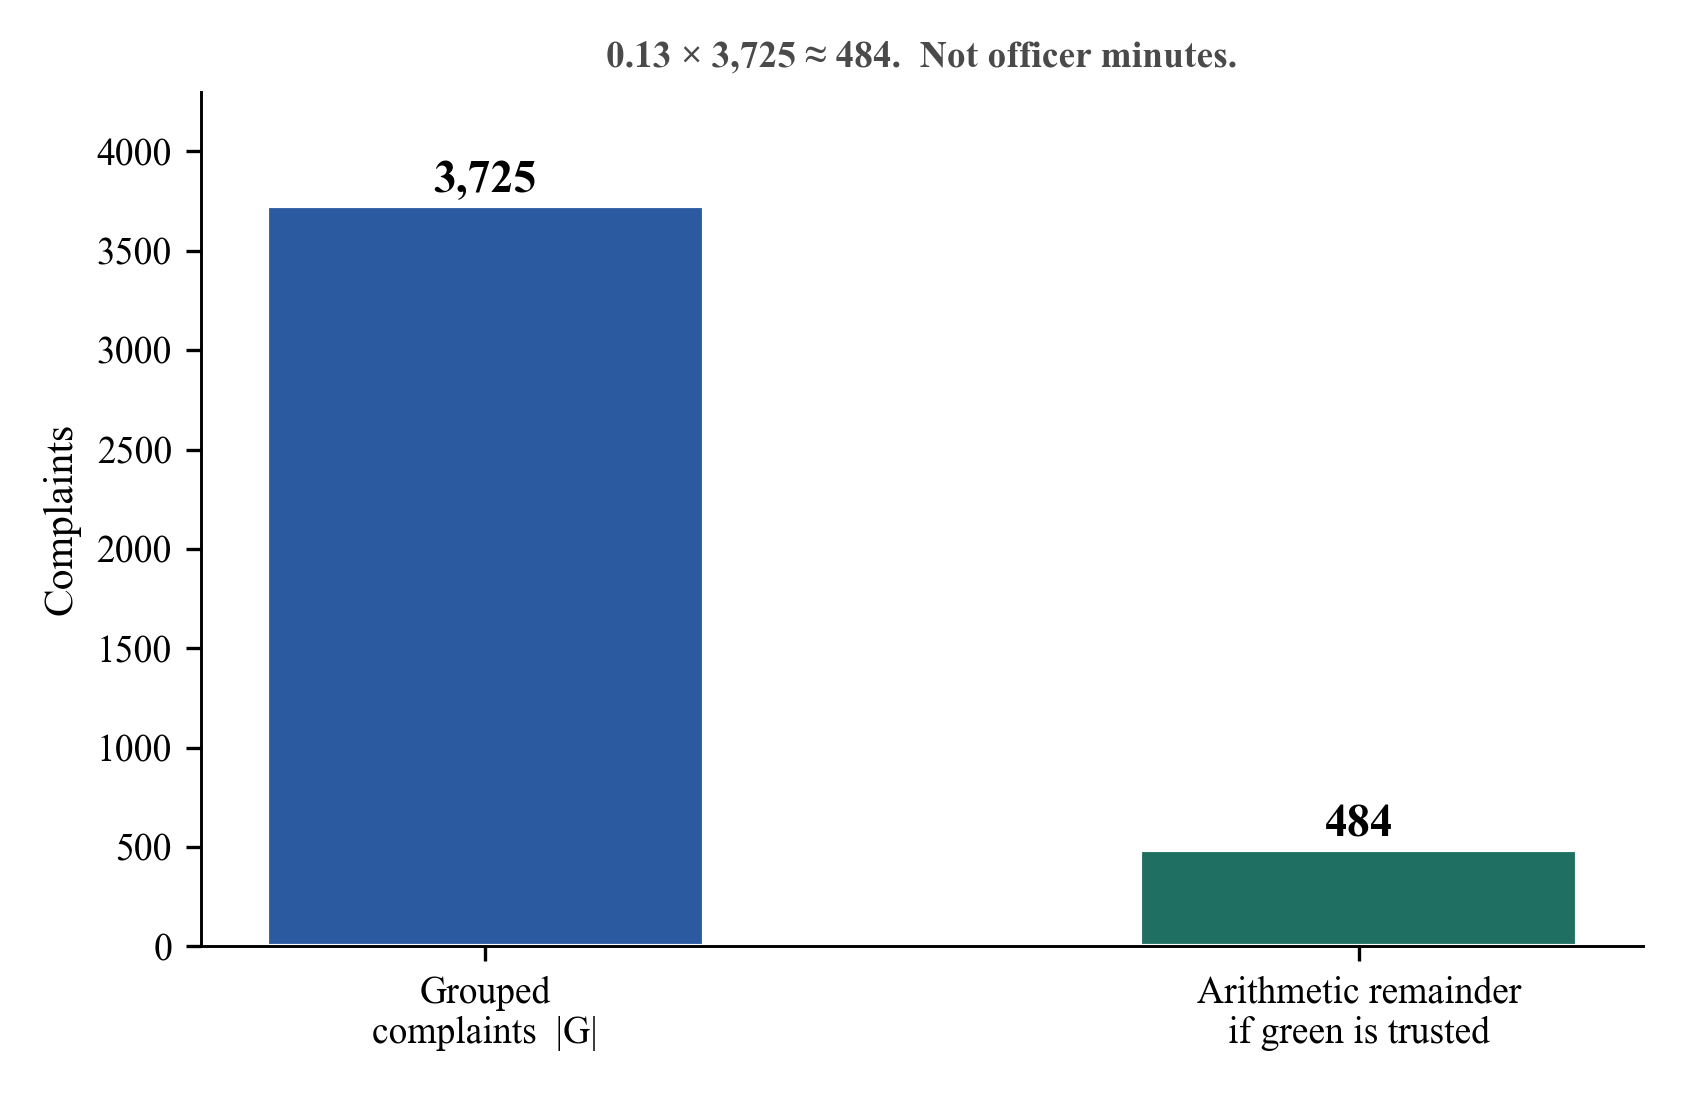
\includegraphics[width=0.72\textwidth]{figures/fig4_operator_load.png}
\caption{Estimated reading load if the green band is trusted.}
\label{fig:load}
\end{figure}

The live TF-IDF job on 28 August 2026 shows a wave day (Figure~\ref{fig:day}): 48 of 49 complaints in one cluster at 08:00; 73 identical texts at 12:00; 127 processed, 124 grouped (97.6\%). That is not in conflict with 62.4\% on the long mixed set.

\begin{figure}[ht]
\centering
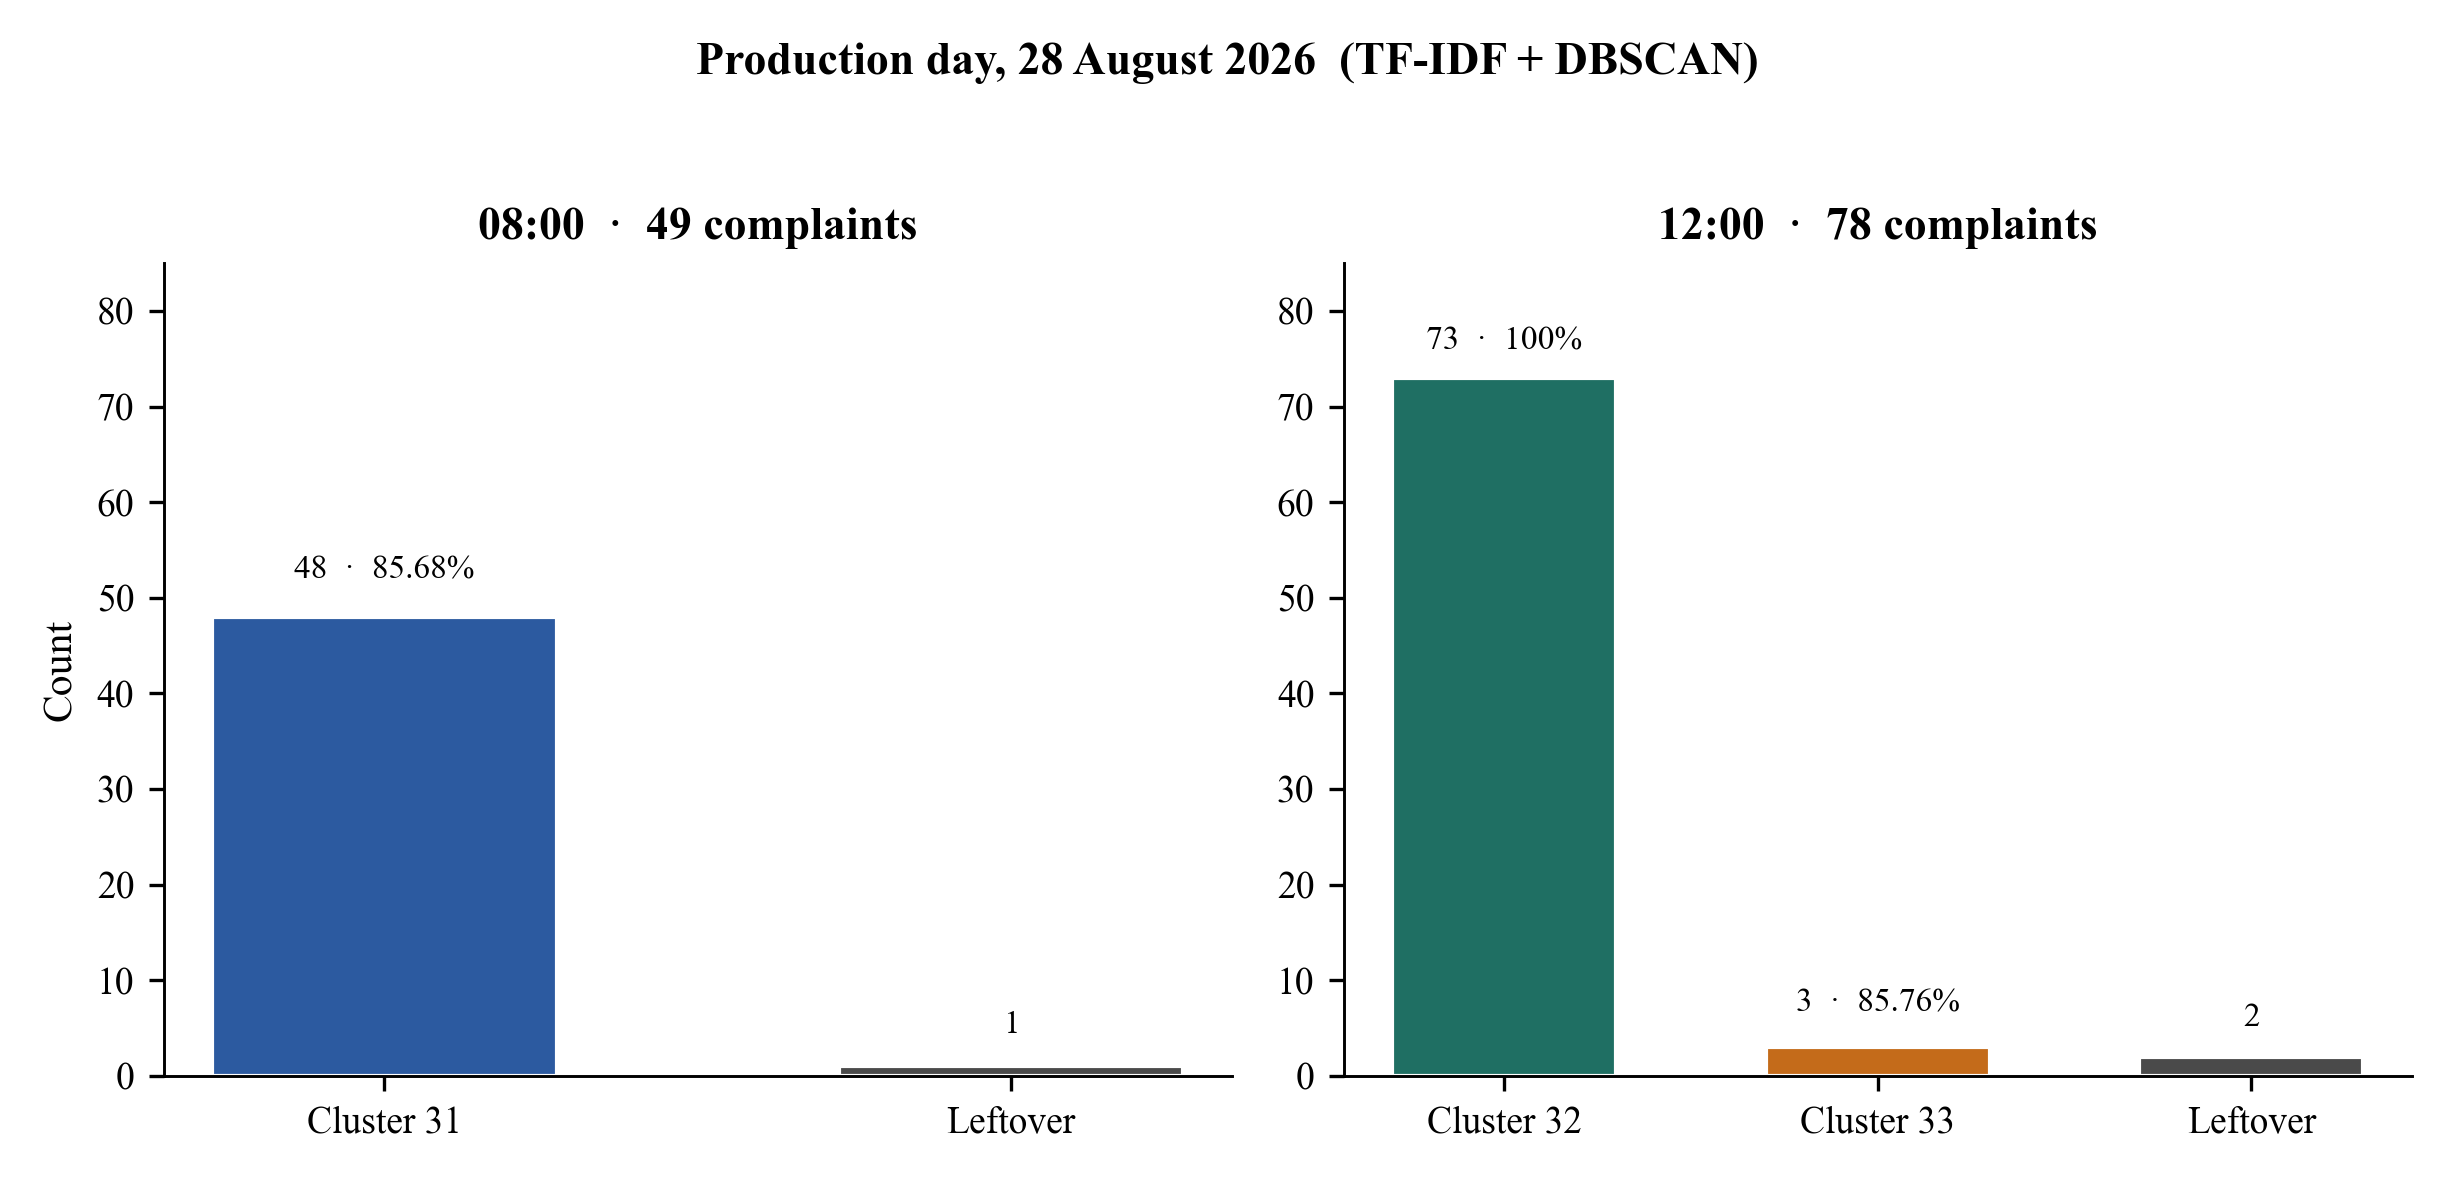
\includegraphics[width=0.92\textwidth]{figures/fig5_production_day.png}
\caption{Production TF-IDF + DBSCAN on 28 August 2026.}
\label{fig:day}
\end{figure}

September 2026 showed the gap between a homolog notebook and Airflow: library blocks, Sentence-Transformers 5.1.2 versus a model saved with 5.4.0, short texts, and a collapse toward one cluster. The 84.9\% figure is a batch result, not the steady daily rate.

\section{Discussion}
Lexical clustering catches copy-paste waves. It fails when two people write the same event in different words. The homolog stack moves the cut from tokens to sense and spends the LLM only on leftovers, following the cost lesson in Rakhimzhanov et al.~\cite{rakhimzhanov2025transport}. The $768 \rightarrow 27 \rightarrow 104$ funnel must be stress-tested: if the 27 candidates already contained the 104, the LLM credit is overstated.

Compared with Esperan\c{c}a et al.\ and Tang et al., the claim here is not a dashboard of themes. It is a count of how many ombudsman files can share one case before a human reads them.

\section{Limitations}
Numbers come from team reports, not a public dataset. COUVI has not labeled a sample. The embedding checkpoint is unnamed. DeepSeek R1 is a moving model. September failures show that 84.9\% is not the current daily truth. We do not measure time saved. Authorship is incomplete.

\section{Ethics, funding, and AI}
Complaint text stays inside CGE. Clustering is an aid; an officer still closes the case. No external grant. The authors work for the agency that operates the system. A language model helped organize the English draft and render the figures. Counts came from team notes. The corresponding author is responsible for every number.

\section{Conclusion}
On 4{,}389 real complaints, TF-IDF + DBSCAN grouped 62.4\%. Embeddings + HDBSCAN + a leftover LLM grouped 84.9\% and recovered 104 leftovers. A wave morning in August grouped 97.6\% of that day's files. The next version needs COUVI labels, a pinned model, and a stable week of production logs.

\begin{thebibliography}{9}
\bibitem{salton1988term}
G.~Salton and C.~Buckley. Term-weighting approaches in automatic text retrieval. \textit{Information Processing \& Management}, 24(5):513--523, 1988. \url{https://doi.org/10.1016/0306-4573(88)90021-0}

\bibitem{ester1996dbscan}
M.~Ester, H.-P.~Kriegel, J.~Sander, and X.~Xu. A density-based algorithm for discovering clusters in large spatial databases with noise. In \textit{KDD-96}, pages 226--231. AAAI Press, 1996.

\bibitem{campello2013hdbscan}
R.~J.~G.~B.~Campello, D.~Moulavi, and J.~Sander. Density-based clustering based on hierarchical density estimates. In \textit{PAKDD 2013}, LNCS 7819, pages 160--172. Springer, 2013. \url{https://doi.org/10.1007/978-3-642-37456-2_14}

\bibitem{reimers2019sbert}
N.~Reimers and I.~Gurevych. Sentence-BERT: Sentence embeddings using Siamese BERT-networks. In \textit{EMNLP-IJCNLP 2019}, pages 3982--3992, 2019. \url{https://doi.org/10.18653/v1/D19-1410}

\bibitem{grootendorst2022bertopic}
M.~Grootendorst. BERTopic: Neural topic modeling with a class-based TF-IDF procedure. arXiv:2203.05794, 2022. \url{https://doi.org/10.48550/arXiv.2203.05794}

\bibitem{das2020grievance}
R.~K.~Das, M.~Panda, and H.~Misra. Decision support grievance redressal system using sentence sentiment analysis. In \textit{ICEGOV 2020}, pages 17--24. ACM, 2020. \url{https://doi.org/10.1145/3428502.3428505}

\bibitem{tang2024bertopic}
Z.~Tang, X.~Pan, and Z.~Gu. Analyzing public demands on China's online government inquiry platform: A BERTopic-based topic modeling study. \textit{PLOS ONE}, 19(2):e0296855, 2024. \url{https://doi.org/10.1371/journal.pone.0296855}

\bibitem{esperanca2025complaint}
M.~Esperan\c{c}a et al. Proactive complaint management in public sector informatics using AI. \textit{Applied Sciences}, 15(12):6673, 2025. \url{https://doi.org/10.3390/app15126673}

\bibitem{rakhimzhanov2025transport}
D.~Rakhimzhanov, S.~Belginova, and D.~Yedilkhan. Automated classification of public transport complaints via text mining using LLMs and embeddings. \textit{Information}, 16(8):644, 2025. \url{https://doi.org/10.3390/info16080644}
\end{thebibliography}

\end{document}
